\documentclass[11pt]{article}
\usepackage[review]{acl}
\usepackage{times}
\usepackage{latexsym}
\usepackage[T1]{fontenc}
\usepackage[utf8]{inputenc}
\usepackage{microtype}
\usepackage{inconsolata}
\usepackage{amsmath,amssymb}
\usepackage{booktabs}
\usepackage{array}
\usepackage{graphicx}

% Research draft: the proposed resource, controller, and evaluation are not results.
\title{Agentic Waterfall: A Framework for Continual Feed Interaction}
\author{Anonymous ACL submission}

\begin{document}
\maketitle

\begin{abstract}
An information feed must continue serving a person as their interests, tasks, and understanding change. A user may explicitly redirect the feed, signal preferences through behavior, or browse without a stated goal. These signals can affect not only the order of available items but also what content should be acquired and what the system should remember. We formulate \emph{Agentic Waterfall Feed} as continual decision-making over content acquisition, recommendation, and user-state maintenance in an interactive feed. We describe a reference agent that receives language, observed behavior, and authorized memory, produces structured actions, and conditions subsequent decisions on execution results and actual exposure. We also propose an episode-based resource and evaluation protocol that separates blind comparisons at a shared interaction prefix from independently evolving user--system trajectories. The protocol covers both goal-directed and open-ended browsing, and treats simulated users as an auxiliary tool whose validity must be tested against held-out human choices. This manuscript presents a research design: the complete controller, dataset, and empirical comparisons remain to be realized, and no effectiveness results are reported.
\end{abstract}

\section{Introduction}
A person using an information feed may start by browsing camera reviews, purchase a camera, and then ask for short tutorials on photographing a football match. The system must recognize that an earlier shopping task has ended while the camera remains relevant. It may search for tutorials, select suitable items it already has, or combine both actions. Later, the user may ask for written instructions instead of videos; an appropriate response changes the current presentation constraint without assuming that the person dislikes photography. Other sessions have no explicit task at all: the person simply browses, and the feed must respond to observed behavior without inventing a specific hidden goal.

These interactions join several problems often evaluated separately. Language conveys requests and corrections, behavior supplies partial evidence about what was actually seen, and user memory carries information across decisions. Acquisition determines which items enter the candidate pool; recommendation determines what reaches the user; and subsequent behavior depends on that exposure. A good next item does not by itself show that the system will remain useful after a change in context, while an attractive static ranking cannot reveal whether an agent can find missing material.

Prior work already addresses important portions of this setting. RecBot incorporates active commands and plans recommendation operations \citep{tang2026recbot}; MARS manages hierarchical user memory \citep{shen2026mars}; and ClawRec connects evidence-based state, source planning, acquisition, curation, and feedback \citep{wu2026clawrec}. Our aim is not to attribute the combination of these components to a new invention. Instead, we use their overlap as motivation to specify the \emph{complete interaction} as a shared object of study: what information is available at each decision, what actions can be taken, and how systems can be compared as their interactions unfold.

We propose three connected parts. First, we define Agentic Waterfall Feed, covering both goal-directed and open-ended browsing, as a continual process that maps language, observed behavior, authorized memory, and environment state to actions. Second, we describe Waterfall, a reference framework for producing and executing structured state, acquisition, and recommendation actions. Third, we propose an episode-based resource and evaluation protocol that combines human blind choices at shared prefixes with separate interactive trajectories. Our central research question is whether systems that manage the full process provide more useful ongoing experiences under comparable information and resource constraints, and which decisions explain the difference. The framework and protocol are proposals, not completed empirical contributions; the full implementation, data collection, and comparisons remain future work.

\section{Related Work}
\paragraph{Language and interactive recommendation.} RecBot studies active user commands within a recommendation feed, parses constraints, and plans tool chains; its evaluation includes offline interactive experiments and an online study \citep{tang2026recbot}. InteRecAgent and iAgent also use language agents to mediate or orchestrate recommendation tools \citep{huang2025interecagent,xu-etal-2025-iagent}. These systems establish that language control and tool use are established research directions. Our task definition places them alongside acquisition, behavior, and memory in a continuing feed, and asks how to evaluate their combined effects.

\paragraph{Memory and complete agent workflows.} MARS represents events, preferences, and profiles in hierarchical memory and uses lifecycle operations to maintain that memory \citep{shen2026mars}. ClawRec is a particularly close comparison: it constructs evidence from behavior, maintains user state, plans across sources, acquires content, and curates recommendations \citep{wu2026clawrec}. Its SimBench evaluates a held-out next step from a history prefix. Our proposed independently evolving trajectory evaluation complements that setting; it does not imply that ClawRec lacks a feedback loop. Any claim of an advantage over these systems requires a fair implementation and empirical comparison.

\paragraph{Interaction data and evaluation.} MIND records news content and impression-level behavior \citep{wu2020mind}, while KuaiRand includes sequential video feedback with random exposures \citep{gao2022kuairand}. Such data support useful ranking and behavioral studies, but a recorded click does not reveal what would have happened had a different agent shown another item. The proposed resource therefore records the environment and execution trace as well as actual exposure and subsequent feedback. Standard ranking metrics such as normalized discounted cumulative gain (nDCG) \citep{jarvelin2002cumulated} remain useful for controlled subproblems, but are not a complete measure of a feed interaction.

\section{Task: Agentic Waterfall Feed}
\label{sec:task}
An episode consists of a sequence of decisions, content exposures, and user responses. At decision time $t$, an agent receives an observation
\begin{equation}
o_t = (c_t, h_{\leq t}, m_t, e_t),
\end{equation}
where $c_t$ is the current language input, possibly empty; $h_{\leq t}$ is the behavior and interaction history available by that time; $m_t$ is the authorized user state and memory; and $e_t$ describes the operational environment, including available candidates, sources, pending actions, and remaining budget. Authorized memory means the information made available for this use, not an assumption that the system observes the user's true preferences. The agent need not insert an entire memory store into every prompt, but access rules must be comparable across evaluated systems.

The agent outputs a set of structured actions $a_t = \pi(o_t)$, subject to tool permissions and budgets. The environment executes valid actions and returns receipts; delivered items may then become exposures, and any observed user responses enter a later history. The next observation contains only information available by that decision point. A planned recommendation, delivery, and actual exposure are distinct events. Underlying utility and future user actions remain unobserved. Updating a runtime state does not entail training or changing the parameters of the language model.

\paragraph{Two modes of use.} Goal-directed browsing can involve an explicit objective, intermediate progress, completion, and a legitimate decision to stop. Open-ended browsing can lack a stated or fixed objective; useful content may offer interest, novelty, or a reason to continue. Neither case requires the agent to elicit an instruction at every step. A longer session is not automatically better, and stopping after a task is fulfilled is not a failure.

\paragraph{What must be decided.} A suitable item may already be in the pool, or a new source query may be necessary. A new utterance can add a task constraint, revise a previous interpretation, or state that a task is complete. Implicit events are less specific: an exposure or short dwell alone does not establish a dislike. These distinctions matter because acquisition, recommendation, and memory affect one another, but they do not establish that a particular controller will outperform existing systems.

\section{Waterfall Reference Framework}
\label{sec:method}
Figure~\ref{fig:agentic-loop} illustrates the proposed interaction loop. Waterfall is a proposed reference implementation of the task interface, designed to make decisions and their consequences inspectable. It can use a language model with frozen parameters, existing retrieval and ranking tools, and a runtime user-state store. The proposal adopts established ideas from prior work rather than treating the interface or its structured encoding as a new learning algorithm.

\begin{figure*}[t]
\centering
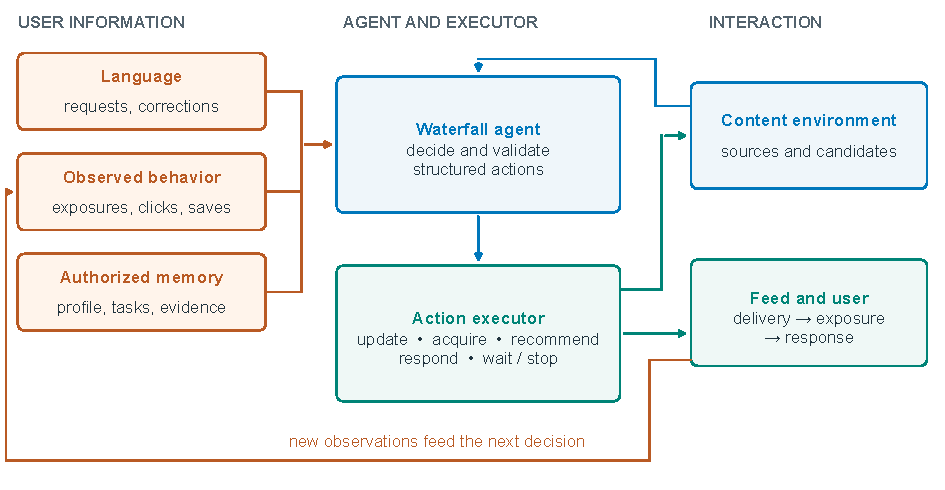
\includegraphics[width=\textwidth]{figures/agentic-waterfall-loop.pdf}
\caption{Proposed Agentic Waterfall loop. Language, observed behavior, and authorized memory inform structured actions. The executor interacts with the content environment and the feed; tool outcomes and user responses inform subsequent decisions. The diagram describes the proposed framework, not an empirical result.}
\label{fig:agentic-loop}
\end{figure*}

\subsection{Inputs and State}
The agent receives three classes of user information: the user's actual words and their referents; time-stamped behavior linked to the items actually exposed; and authorized profile or memory records. Each state record may include its scope, status, and supporting evidence. A current task constraint can be distinguished from a durable preference; uncertainty and contradictory evidence can be retained. System-side observations include candidate metadata, source capabilities, tool responses, and unfinished actions. Failure to retrieve from a source is an execution outcome, not a negative user preference.

The event representation preserves measurement semantics. A visible card, a click, and video playback are separate events; a missing duration stays missing. A response is associated with the actual exposure where possible, and a later interpretation does not change what the agent knew at an earlier decision. An authorized state update may record an explicit request or a qualified hypothesis, but a single interaction need not become a lasting preference.

\subsection{Actions and Execution}
The agent can request any compatible combination of five action types:
\begin{itemize}
\item \textsc{UpdateState}: add, revise, retire, or retain a scoped state record, with evidence and an operation;
\item \textsc{Acquire}: query authorized sources with explicit source, query, content type, and limits;
\item \textsc{Recommend}: select and order available item identifiers for delivery;
\item \textsc{Respond}: communicate or ask a relevant question; and
\item \textsc{Idle}: wait, keep the current state, or stop a completed task.
\end{itemize}
Each request carries an identifier, parameters, evidence references when applicable, and explicit dependencies. The executor validates the action type, allowed sources, arguments, referenced items, and dependencies. Independent acquisitions may run concurrently; a dependent recommendation waits for the required results. Invalid actions are recorded with their errors, and successful calls return receipts containing actual results or failure. A recommendation receipt records what was queued, not what was seen. Late results are reconsidered against current state before use. The exact controller, prompts, thresholds, and tool implementations must be fixed and reported before evaluation.

\subsection{Illustrative Interaction}
Suppose the user says: ``I bought the camera; show me short guides for filming football.'' The input contains the utterance, the earlier observed browsing events, an authorized memory of the camera, and the current pool and source capabilities. A valid output can finish the shopping task, open a filming task with a short-format constraint, and request two independent searches for articles and videos. If the searches require the new task state, both declare that dependency; after it is applied, the searches can execute in parallel. Once their results return, the next decision can recommend actual returned identifiers. If the user then says ``written steps only,'' the agent updates the task constraint and can reorder suitable available articles or acquire more. It should not infer a general dislike of videos from a task-local request. The example is authored for exposition; it is not an observed study episode.

\section{An Episode-Based Resource}
\label{sec:resource}
We propose a resource for comparing complete systems rather than only their outputs on a fixed candidate set. An episode records an initial authorized context, a versioned content environment, subsequent user inputs, decisions, tool results, delivered items, actual exposures, and responses. The environment should allow systems to issue their own queries under a common snapshot, tool interface, and budget. Different systems may therefore retrieve different items. A resource is reproducible only to the extent that the underlying content, indexes, and permissions can be preserved or reconstructed.

\paragraph{Data objects.} Each episode should store (1) pseudonymous participant and episode identifiers, provenance and consent references; (2) content identifiers, source, modality, availability time, snapshots or verifiable references, and near-duplicate groups; (3) decision-time inputs, state versions, raw and parsed actions, validation, execution receipts, and costs; (4) ordered deliveries and actual exposure identifiers, positions, timestamps, and observed feedback; and (5) evaluation choices and labels kept separate from policy inputs. Where content cannot legally be redistributed, a reference and hash can document it, but an inaccessible snapshot limits replay. Missing fields must remain missing. Collected, author-created, controlled, and simulated episodes must be identified separately.

\paragraph{Time and leakage.} Event time and the time information became available to the system are recorded separately. No future command, later annotation, hidden evaluation choice, or feedback on another system's item may enter a policy's current observation. The archive can contain all these objects for audit, but a runtime must construct the agent input through a restricted interface. Participants and derivatives of the same underlying episode must remain within the same data split. Only actually known randomization probabilities should be recorded; observational logs alone do not supply counterfactual responses.

\paragraph{Collection plan.} A human-facing feed would record natural language, actions, and actual exposure under consent, with goal-directed and open-ended sessions and cold-start cases. Controlled scenarios may supplement naturally arising changes, but are labeled as such. A small pilot should check whether the interface, content supply, exposure capture, and evaluation questions work before the formal protocol and sample size are fixed. No participants have yet been recruited or data collected for this proposed resource.

\section{Evaluating the Complete Feed}
\label{sec:evaluation}
We separate a shared-prefix comparison from a continuing-use comparison. Each answers a different question, and neither should be substituted for the other. Figure~\ref{fig:human-evaluation} summarizes the two protocols.

\begin{figure*}[t]
\centering
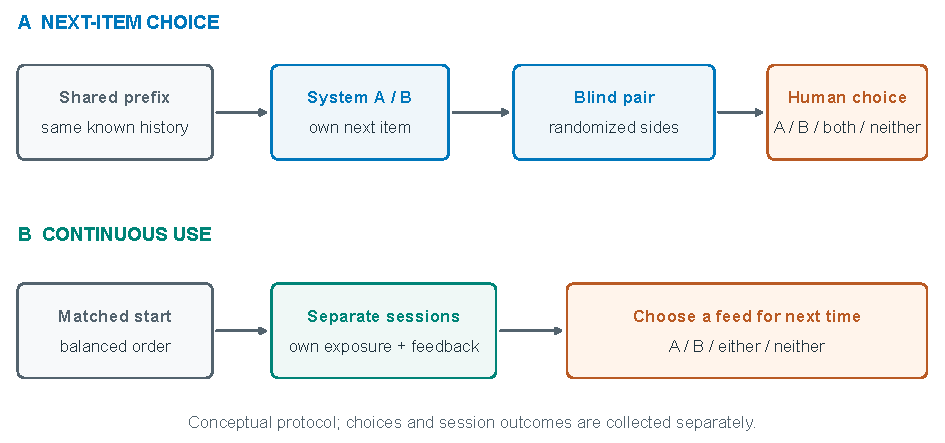
\includegraphics[width=\textwidth]{figures/agentic-waterfall-evaluation.pdf}
\caption{Proposed human evaluation. (A) At a shared prefix, systems independently propose a next item for a randomized blind choice. (B) Participants use systems in separate sessions and choose which feed they would use again. The protocols are design proposals; no outcomes have been collected.}
\label{fig:human-evaluation}
\end{figure*}

\subsection{Which Next Item Would the Person Choose?}
At a frozen interaction prefix, two systems receive the same permissible information and access to the same content environment. Each proposes its next item under a specified budget. The participant sees the two items with anonymous, randomized positions and chooses the one they would prefer to view, a tie, or neither. If both systems select the same item, the trial is recorded as identical rather than treated as evidence for one system. Each choice is held outside the policy input for this comparison.

For nonidentical pairs, we propose reporting the fraction of trials won by each system, ties, and neither choices, together with the number of identical pairs and participant-level uncertainty intervals. The unit of uncertainty must account for repeated decisions from the same person. A forced two-way win rate alone would hide cases where neither result is useful; the full distribution preserves that information. For longer slates, the presentation and choice question must be specified in advance instead of treating one item as a substitute for a whole session.

\subsection{Which Feed Is Better to Use Over Time?}
In a separate interactive study, a participant uses each assigned system in a counterbalanced order or under another pre-specified assignment. Each system receives only feedback generated by its own exposures and maintains its own state. After comparable sessions, the participant can report which feed they would prefer to continue using, or indicate a tie or neither. Goal-directed sessions additionally record whether the participant reports meaningful progress or completion; exploratory sessions ask whether content was worth viewing and offered useful discoveries. The comparison should record unequal exposure and legitimate early task completion rather than penalizing the system for not filling a fixed number of slots.

This protocol estimates experience within the observed session and study population. It does not establish long-term retention or real-world outcomes outside that period. Because a live trajectory changes with each system's earlier choices, the outcomes cannot be assembled by concatenating the winners of independent next-item comparisons. Task order, carryover, repeated content, and different starting conditions require explicit control and reporting.

\subsection{Diagnostics and Standard Metrics}
Besides human choices, report constraint violations, response to an explicitly stated change, invalid actions, latency, model and source calls, and state changes supported by evidence. These are diagnostic measures, not a single subjective total score. State and action labels require a documented annotation scheme and adjudication; multiple action paths may be acceptable.

For a fixed labeled candidate set, nDCG compares a system's ranked gain with the ideal ranking for that same set \citep{jarvelin2002cumulated}. For example, if relevant grades are $2,1,0$, the gain at each rank is discounted by position, and the resulting sum is divided by the best possible sum for those grades. This measures ranking under the chosen labels and candidate pool; it does not measure a system's ability to acquire missing content or its effect on later behavior. Existing datasets such as MIND and KuaiRand can provide controlled subtask checks with their original signal semantics, not fabricated language or counterfactual interactions.

\subsection{Simulated Users}
Simulated users could make wider comparisons affordable, but their responses are not assumed to stand in for people. A simulator must receive only the permitted profile and the history and items produced in its own trajectory. It should be evaluated on held-out human choices, agreement about system ordering, and responses to changes across relevant scenarios and user groups. Development and test participants and their derived simulations must be separated. Simulated results are reported independently and support conclusions only within the range for which agreement has been demonstrated.

\section{Research Questions and Comparisons}
The proposed experiments ask: (1) whether the complete feed improves next-item and session-level human choices; (2) whether coordinated language, behavior, acquisition, and memory contribute beyond strong alternatives; and (3) where offline ranking and simulated responses agree or diverge from human judgments. These questions are open. The comparison set should include a continuously run ClawRec adaptation with its normal state update and replanning abilities, a strong general tool-using agent given the same information, and a reasonable combination of established command, memory, and retrieval components. RecBot- or MARS-inspired implementations should be labeled as paper-based adaptations when official implementations cannot be verified. A fixed-pipeline baseline and controlled removal of individual inputs or action capabilities provide additional diagnosis.

Models, available information, content environment, tool opportunities, budgets, and evaluation questions should be matched where feasible, with unavoidable differences disclosed. Candidate pools may differ because acquisition is part of the task. A system must not receive feedback on items that it did not actually show, and comparisons should not weaken a baseline by preventing a capability it normally has. Before a formal test, the study must freeze prompts, models, tool versions, allocation and ordering, episode splits, primary outcomes, and an analysis plan informed by the pilot.

\section{Empirical Status and Discussion}
The present manuscript specifies a task, a reference framework, and a proposed resource and evaluation. It does not report a completed dataset, validated simulator, comparative human study, or quantitative result. Existing product components and a local demonstration are not evidence that the full research controller or its evaluation has been implemented. The next scientific step is to build and pilot the common environment and collect actual interactions, then run the strong comparisons with the study protocol fixed. Depending on those results, the eventual contribution may lie in the task and resource, the method, empirical findings, or a combination; the outcome cannot be decided from the design alone.

\section{Conclusion}
Agentic Waterfall Feed frames continued information consumption as a sequence of decisions over acquisition, recommendation, and user-state maintenance. Waterfall provides a proposed structured interface for those decisions, while the episode-based evaluation asks people both which next item they prefer and which system they prefer after use. Together, these proposals make the complete interaction testable; their practical value and distinction from strong existing agents remain empirical questions.

\section*{Limitations}
This is a research design without completed comparative evidence. A short controlled session cannot establish long-term value, and a frozen content snapshot may omit changing source availability or new content. Human preference can depend on presentation, task order, content familiarity, and participant population; a blind choice does not by itself measure task completion. Language-model-based simulation can reproduce its assumptions rather than human behavior. Achieving comparable tools and budgets across systems may require adaptations that change their original behavior, and any such changes must be disclosed. Finally, the reference action interface does not guarantee correct reasoning or prove that a specialized controller is necessary.

\section*{Ethics Statement}
The proposed study involves user behavior, language, and potentially sensitive profile information. Before collection, the researchers must determine the applicable institutional review and data-protection requirements, obtain appropriate consent, and define access, retention, deletion, and publication procedures. Participants should be able to avoid disclosing sensitive information. Data and content may be shared only under applicable consent and rights; this draft does not claim approval or permission to release them.

\bibliography{waterfall}
\end{document}
